\section{Results}
\label{sec:results}

We report three kinds of evidence. The hidden Kaggle score is the only one free of contamination. A same-server
comparison with the Duck harness isolates the agent from the hardware. Run telemetry shows where the time and the
tokens go. Section~\ref{sec:method} describes the current code. The runs below used earlier builds of it, and we say
where a difference matters.

\subsection{The hidden-set trajectory}

\begin{figure*}[t]
\centering
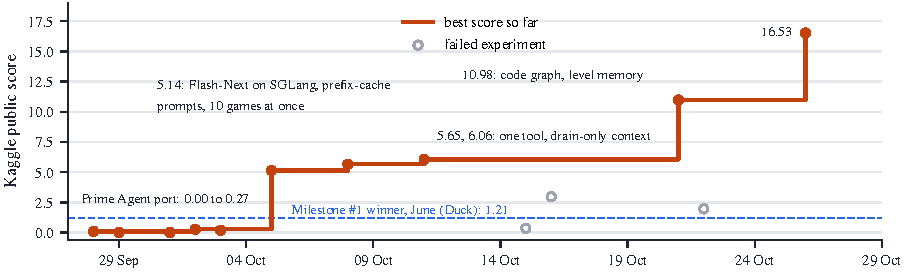
\includegraphics[width=\textwidth]{figures/leaderboard.pdf}
\caption{Every completed submission of our team to the Kaggle ARC-AGI-3 leaderboard (hidden games), with the main
change in each build. Hollow points are experiments that made things worse. They are kept on the plot, and each one
was rolled back. Four further submissions failed with Kaggle system errors during the rerun and have no score.}
\label{fig:leaderboard}
\end{figure*}

Figure~\ref{fig:leaderboard} shows the whole trajectory. The faithful port of Prime Agent's harness to open
weights scored 0.00--0.27. The model wrote code, but it brute-forced: in one 10-game run it reset 350 times and never
found a goal. Moving to Qwen3.8-Flash-Next on SGLang, with prompts laid out for the prefix cache and ten games at once,
took the score to 5.14. Merging the move tool into the Python tool and switching to drain-only context gave 5.65 and
6.06. The code graph, memory keyed by level and the one-request turn cycle gave 10.98. The current build, with
Duck-style draining and the briefing map switched back on, scored \textbf{16.53} on 26 October. That is 24 days after
0.27, and 13.7$\times$ the 1.21 that won Milestone~\#1 in June.

The field did not stand still. On the day we submitted, the leading entry scored 71.48, Tufa Labs' own current entry
68.91, and the 200th entry 32.69. In absolute terms \textsc{Sarbloh} is not competitive with these teams, and we do not
claim it is. What we claim is narrower: the curve, the engineering that produced it, and the parts of it that transfer.

\subsection{Same server, same model: against the Duck harness}

\begin{figure}[t]
\centering
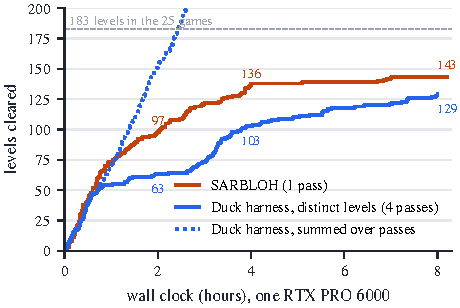
\includegraphics[width=\columnwidth]{figures/levels_vs_time.pdf}
\caption{Levels cleared over wall-clock time on the 25 public games, both agents on the same SGLang server and the
same Flash-Next weights. The Duck harness ran four passes of every game at once (100 runs). Solid blue counts a level
once per game, dotted blue counts it every time a pass clears it.}
\label{fig:curves}
\end{figure}

To separate the agent from the hardware, we ran a later release of the Tufa Labs Duck harness than the June winner on
\emph{our} server, with identical SGLang arguments and the same model. It played four passes of each public game
concurrently. Figure~\ref{fig:curves} compares it with our best single-pass run. \textsc{Sarbloh} clears 73 levels in
the first hour against 54, 97 against 63 at two hours, 136 against 103 at four, and 143 against 129 at 8.2 hours (of
183). Per GPU-hour the two agents are roughly equal: one Duck pass, which held about a quarter of the GPU, reached
about 104 levels. Our advantage is that the scheduler spends the same GPU on the games most likely to score next
rather than on four copies of each, so distinct levels arrive earlier. That matters under a hard nine-hour limit.

Figure~\ref{fig:pergame} breaks this down by game. With one pass against the Duck's best of four, \textsc{Sarbloh}
clears more levels in eight games, the largest gaps being \code{sk48} (8 against 0), \code{lf52} (6 against 1),
\code{wa30} (7 against 2) and \code{g50t} (6 against 3). The Duck does better in four (\code{tn36}, \code{vc33},
\code{s5i5}, \code{sp80}), and thirteen are tied. Both agents stall in \code{bp35}.

\begin{figure*}[t]
\centering
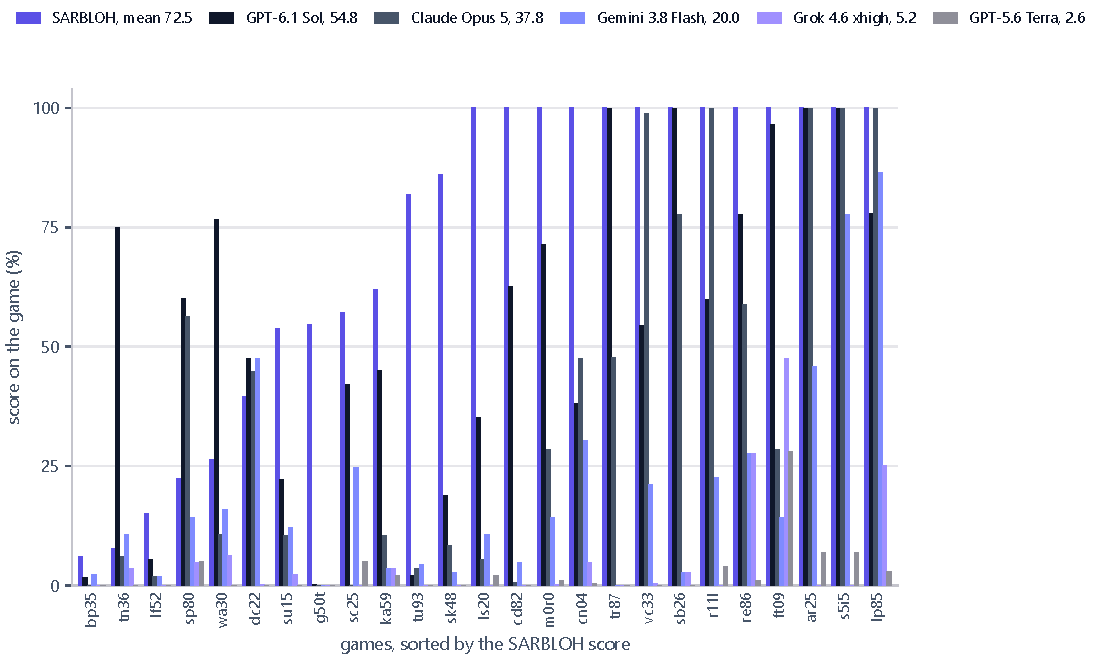
\includegraphics[width=\textwidth]{figures/per_game.pdf}
\caption{Levels cleared per public game: our single pass against the Duck harness's best of four passes, on the same
server. Games are sorted by our completion rate.}
\label{fig:pergame}
\end{figure*}

\subsection{Efficiency once a level is understood}

RHAE punishes every action quadratically, so we also measure how efficient the agent is on the levels it clears.
In the best run the \emph{median} cleared level took 0.77 of the human baseline's actions, which earns the 1.15 cap
(Eq.~\ref{eq:rhae}). Once the agent understands a level it plays it at or above human efficiency: it reasons in code
and sends the path. Taking the run's 59.4 mean public-game score as a reference (a development number on
contaminated games), the 40.6 points it lost split roughly into 12.6 from extra actions on cleared levels, 8.0 from 13
levels attempted but not solved, and 19.5 from levels never reached because a game stalled earlier. Most of the loss is
not inefficiency. It is levels the agent never came to understand.

\subsection{Where the GPU time goes}

\begin{table}[t]
\centering
\small
\begin{tabular}{@{}lr@{}}
\toprule
Measure (9-hour run, 25 games, one GPU) & Value \\
\midrule
Prompt tokens served from the prefix cache & \textbf{98.4\%} \\
Prompt tokens / reply tokens & 1.78\,B / 14.4\,M \\
Model calls / LLM failures & 21,224 / 0 \\
Games inside a turn at once (mean) & 11.8 \\
Turns per minute, all games & 42.7 \\
Decode speed per request & 76 tok/s \\
Turn wall time, median / p90 & 2.3\,s / 30.2\,s \\
Busy time decoding / prefilling & 50.1\% / 1.3\% \\
Share of reply text that is thinking & 78\% \\
Minutes per cleared level (median) & 9.2 \\
Actions / human baseline, cleared levels (median) & 0.77 \\
\bottomrule
\end{tabular}
\caption{Telemetry of the best offline run (143/183 levels), from the harness's own speed report.}
\label{tab:telemetry}
\end{table}

Table~\ref{tab:telemetry} shows that the system is decode-bound, which is what we designed for. Prefill takes 1.3\%
of busy time because 98.4\% of all prompt tokens are reused from the cache. Before the append-only rewrite, the same
agent reused about 10\% and prefill starved every other game. The server made 21,224 calls with no failures in nine
hours.

\subsection{What the numbers do not show}

\paragraph{The briefing has not been isolated.} The 143-level run sent the lettered board and the plain picture, with
the briefing and the map switched off. The 16.53 build had both switched on. Other changes landed between those builds,
so neither number measures the briefing alone. What the briefing does have is the lab evidence (\S\ref{sec:lab}) and
the oracle result (\S\ref{sec:motivation}). A same-model A/B on the hidden set is the next experiment.

\paragraph{Failure modes.} Thirteen levels were attempted and never solved. \code{bp35} and \code{sp80} stopped at level
2 in every full run we made. In the best run, four games came 2--15 moves short of the 2,000-action cap and the model
then answered ``\code{Holding...}'' to the continue prompt about 14,000 times, which burned 1.24\,B of the 1.78\,B
prompt tokens on turns that did nothing. The current build caps each game at 400 turns, which bounds such a stall. Finally, a negative result:
replacing old code in the history with a one-line stub, to save tokens, made the model write the stub \emph{as its
code} in 97.7\% of its calls, and the run cleared no level. A small model copies what it sees.
